% TEMPLATE for Usenix papers, specifically to meet requirements of
%  USENIX '05
% originally a template for producing IEEE-format articles using LaTeX.
%   written by Matthew Ward, CS Department, Worcester Polytechnic Institute.
% adapted by David Beazley for his excellent SWIG paper in Proceedings,
%   Tcl 96
% turned into a smartass generic template by De Clarke, with thanks to
%   both the above pioneers
% use at your own risk.  Complaints to /dev/null.
% make it two column with no page numbering, default is 10 point

% Munged by Fred Douglis <douglis@research.att.com> 10/97 to separate
% the .sty file from the LaTeX source template, so that people can
% more easily include the .sty file into an existing document.  Also
% changed to more closely follow the style guidelines as represented
% by the Word sample file. 

% Note that since 2010, USENIX does not require endnotes. If you want
% foot of page notes, don't include the endnotes package in the 
% usepackage command, below.

% This version uses the latex2e styles, not the very ancient 2.09 stuff.
\documentclass[letterpaper,twocolumn,10pt]{article}
\usepackage{usenix,epsfig,endnotes,listings,subfig}
\begin{document}

%don't want date printed
\date{}

%make title bold and 14 pt font (Latex default is non-bold, 16 pt)
\title{\Large \bf An Untitled Paper About Determinism}

%for single author (just remove % characters)
\author{
%{\rm Your N.\ Here}\\
%Your Institution
%\and
%{\rm Second Name}\\
%Second Institution
% copy the following lines to add more authors
% \and
% {\rm Name}\\
%Name Institution
} % end author

\maketitle

% Use the following at camera-ready time to suppress page numbers.
% Comment it out when you first submit the paper for review.
\thispagestyle{empty}

\newcommand{\checkout}{{\tt checkout()}}
\newcommand{\settled}{{\tt commit()}}
\newcommand{\settledm}{{\tt commit\_mutex()}}
\newcommand{\update}{{\tt update()}}
\newcommand{\updatem}{{\tt update\_mutex()}}
\newcommand{\commit}{{\tt commit()}}
\newcommand{\commitm}{{\tt commit\_mutex()}}
\newcommand{\mksnap}{{\tt commit()}}
\newcommand{\getsnap}{{\tt update()}}
\newcommand{\fork}{{\tt fork}}
\newcommand{\pte}{{\tt pte}}
\newcommand{\determEnd}{{\tt determ\_end}}
\newcommand{\pthread}{{\tt pthread}}


\newcommand{\create}{{\tt pthread\_create}}
\newcommand{\dthreads}{Dthreads}



\newcommand{\conversion}{{\sc \small Conversion}}
\newcommand{\lib}{{\sc \small JJT}}

\subsection*{Abstract}

We present \lib{}, a high performance deterministic multi-threading library built on top of version controlled memory.

\section{Introduction}

With multi-core processors comes the need for parallel programs. 
%Along with the profusion of multi-core processors over the last decade has come the need for parallel software that can take advantage of these new architectures. 
%Unfortunately, writing parallel software that is both correct and performs well is hard still an open challenge. 
%Writing sequential software that is correct and performs well is hard enough.
Unfortunately, writing parallel programs is hard. 
On top of the difficulties of writing correct sequential programs, parallelism brings nondeterminism which undermines our ability to debug, test and understand our programs.

%In recent years many researchers have proposed ways to execute general parallel programs deterministically without sacrificing much parallelism or performance. 
Research into deterministic concurrency seeks to alleviate these problems. %has seen much progress in recent years.
While some initial proposals focused on the design of deterministic multi-core architectures \cite{devietti_dmp:_2009,devietti_rcdc:_2011,derek_r._hower_calvin:_2011}, subsequent work has demonstrated practical pure-software implementations of determinism  \cite{liu_dthreads:_2011,merrifield_conversion:_2013,kai_lu_efficient_2014}.

One of the central techniques for improving performance in both hardware and software deterministic systems has been relaxing the memory consistency model. While initial proposals adopted strong consistency models like sequential consistency \cite{devietti_dmp:_2009} and total store order (TSO) \cite{bergan_coredet:_2010}, subsequent work relies on extremely relaxed consistency models like DRF0 \cite{devietti_rcdc:_2011} and lazy release consistency (LRC) \cite{kai_lu_efficient_2014} to reduce inter-thread communication and thus improve performance.
%for good performance.% Weakening the consistency model admits better scalability by allowing memory fences to coordinate with a subset of threads instead of with all threads \cite{devietti_rcdc:_2011,kai_lu_efficient_2014}. 
%Relaxed consistency allows fences to perform localized work instead of the global coordination required by strong consistency models. 
However, all deterministic execution systems, relaxed consistency or not, require global ordering of inter-thread communication, a likely bottleneck in any deterministic concurrency system. 
%This can be abstracted as a deterministic logical clock (DLC), based on synchronization operations \cite{liu_dthreads:_2011} or instruction counting \cite{olszewski_kendo:_2009, devietti_dmp:_2009}, where the thread with the lowest clock has priority.
%Our system, \lib, also implements a deterministic logical clock which inherently requires global coordination (\S\ref{s:dlc}). 
%Our insight is that optimizing the implementation of memory fences is of limited benefit when other global bottlenecks remain. 
We argue that while this bottleneck remains, relaxing the consistency model is of limited benefit. 
Moreover, the adoption of an extremely relaxed consistency model is not free. Supporting LRC, as \cite{kai_lu_efficient_2014} does, suffers from high space overheads that hinder scalability. The programmability challenges inherent in relaxed consistency are also well-known, and can result in unintuitive behavior \cite{adve_data_2010,batty_mathematizing_2011}. Finally, some current hardware memory consistency models like x86 are not as relaxed as LRC. Moving to a weaker consistency model breaks compatibility with existing binaries. In contrast, a system that offers consistency guarantees compatible with modern architectures can support legacy binaries simply by replacing the pthreads library.

% The core issue is that a program that "works" on TSO can break on LRC. Consider flag-based synchronization with locking where the sender uses lock A and the receiver uses (by mistake) lock B. Due to the global nature of commits, this will still work on TSO but will deadlock on LRC. There's a data race in the program so any semantics are permissible, but there is a practical consideration as well that we shouldn't break code that already works.

\lib demonstrates that a deterministic implementation of TSO, a relatively strong consistency model that is compatible with all modern hardware platforms, can perform well across a range of workloads. The primary contributions of this paper are:
\begin{itemize}
%\item We identify that deterministic synchronization is a global bottleneck affecting all deterministic execution schemes, regardless of consistency model.
\item We describe several TSO-compatible optimizations that target the same scenarios that relaxed consistency optimizes, reducing the scope for further improvements from relaxed consistency.
\item We demonstrate deterministic adaptation to program behavior as a means of further improving performance.
%\item We describe a novel implementation of deterministic locking that supports blocking instead of polling.
\item We describe novel implementations of deterministic synchronization operations that are flexible and increase the parallelism of prior techniques.
\item Finally, we demonstrate a deterministic implementation of TSO that achieves a 2.8x and 2.2x improvement over DThreads \cite{liu_dthreads:_2011} and DWC \cite{merrifield_conversion:_2013} (respectively) on the five most challenging benchmark programs.

\newpage

\end{itemize}
While determinism can simplify parallel programming, using complicated memory consistency models to make determinism fast under-cuts these programmability gains. \lib erases this tension by combining determinism and strong memory consistency.

% PLACE HOLDER UNTIL WE HAVE A BETTER PRETTY CONCLUDING PARAGRAPH... 
% Below, we describe and motivate the \lib{} design (\S\ref{s:perf}) and several key optimizations (\S\ref{s:optimizations}). \S\ref{s:sync} describes our deterministic synchronization operations, followed by evaluation (\S\ref{s:eval}), related work (\S\ref{s:related}) and conclusions (\S\ref{s:concl}). 

%%% Local Variables: 
%%% mode: latex
%%% TeX-master: "paper.tex"
%%% End:








% ======= STORE/BOX LISTINGS =======



\newsavebox{\mutexUnlock}
\begin{lrbox}{\mutexUnlock}% Store second listing
\begin{lstlisting}
void mutexUnlock(lock_t* l){
	clockPause();
	waitToken();
	lockRelease(l)
	if (!queueEmpty(l->waitQueue)){
		int tid=remove(l->waitQueue);
		wakeupThread(tid);
	}
	convCommitAndUpdateMem();
	releaseToken();
	clockResume();
}
\end{lstlisting}
\end{lrbox}

\newsavebox{\codeSample}
\begin{lrbox}{\codeSample}% Store second listing
\begin{lstlisting}
int x=0;
void * run (void * arg){
	if (x==1)
		x++;
}
int main(){
	x=1;
	pthread_t t1,t2;
	pthread_create(&t1,NULL,run,NULL);
	pthread_create(&t2,NULL,run,NULL);
	pthread_join(t1,NULL);
	pthread_join(t2,NULL);
}
\end{lstlisting}
\end{lrbox}


%\begin{figure}
%\hspace*{.5cm}
%\usebox{\codeSample}
%\caption{A simplified implementation of token acquisition and release.}
%\label{f:waitToken}
%\end{figure}


\section{Synchronization Primitives}
\label{s:sync}

\lib{} supports deterministic versions of mutual exclusion, conditional variables and barriers. As in previous systems \cite{olszewski_kendo:_2009,kai_lu_efficient_2014}, \lib{} uses the GMIC to deterministically order synchronization along with thread creation, exit and join events. Once a thread becomes the GMIC, it is eligible to acquire the \emph{global token} which is required to perform any deterministic event. The token is useful as both an abstraction for maintaining determinism as well as a means of relaxing the traditional GMIC invariant, necessary to perform the coarsening optimization (see \S\ref{s:optimizations}).


\subsection{Mutual Exclusion}

In Kendo \cite{olszewski_kendo:_2009}, in order to ensure progress for others and to avoid introducing deadlocks, a GMIC thread that failed to acquire a lock would repeatedly increment their logical clock by some value until they were no longer the GMIC. This approach suffers from two problems: 1) the choice of a sensible value to add to the clock while polling requires program-specific tuning and 2) many polling requests to check whether there is a new GMIC thread to notify adds needless latency. A better approach would allow the GMIC thread to block and wait for the lock to be released while continuing to ensure progress for others. We accomplish this by adding the ability for a thread to remove itself from GMIC consideration through the $clockDepart()$ function. 

The $mutexLock()$ implementation (shown in Figure \ref{f:mutexLock}) begins by pausing the clock and acquiring the token via the $waitToken()$ function (shown in Figure \ref{f:waitToken}). If the lock is available (Figure \ref{f:mutexLock}, line 6), the thread commits its changes to memory and begins executing its critical section. However in the case of a held lock (Figure \ref{f:mutexLock}, line 10) the thread will remove itself from consideration for the GMIC and add itself to the lock's queue of waiters.

\begin{figure}
\hspace*{.5cm}
\usebox{\mutexUnlock}
\caption{mutexUnlock() implementation.}
\label{f:mutexUnlock}
\end{figure}


Figure \ref{f:mutexUnlock} shows the implementation of $mutexUnlock()$. After pausing the clock and acquiring the token, we check to see if there are any threads waiting for the lock (Figure \ref{f:mutexUnlock}, line 5). If so, we remove the thread from the wait queue and invoke $wakeupThread()$ which activates the thread using a (non-deterministic) conditional variable and adds the thread back into consideration for the GMIC. \footnote{Our simplified code in Figure \ref{f:mutexUnlock} does not handle one case of potential non-determinism. If the newly activated thread is the GMIC, then we must pass the token to them directly to avoid potential non-determinism with the thread that was the GMIC thread prior to activation.}

Note that, unlike in Kendo \cite{olszewski_kendo:_2009}, $mutexUnlock()$ must acquire the token, as it performs a commit. Kendo assumes that applications are data-race-free and thus enforces no isolation between threads.




%Activating a thread in the manner described thus far can create a non-deterministic schedule. For example, a thread $T1$ with a logical clock $n$ is currently the GMIC and is waiting for the token to be released (line 7 of Figure \ref{f:waitToken}). If another thread $T2$ with a logical clock value of $n-1$ is activated by thread $T3$ using $wakeupThread()$ - once thread $T3$ releases the token it can be acquired by either $T1$ or $T2$. To resolve this non-determinism we add an additional shared variable: the \emph{activation sequence number}. Whenever a token-holder activates another thread (both when unlocking a mutex and signaling with a conditional variable), the sequence number is incremented (line 6 of Figure \ref{f:mutexUnlock}. After acquiring the token a thread must check that the sequence number has not changed (line 10 of Figure \ref{f:waitToken}); and if it has the thread must call $clockIsGlobalMinimum()$ again to ensure it is still the GMIC. 

The techniques described above are also used to support deterministic conditional variables.

\subsection{Barriers}

\lib{} takes advantage of barrier semantics and \conversion{}'s parallel commit feature to improve performance. This is not to be confused with prior synchronous deterministic systems, which used \emph{internal} barriers to perform commits from different threads in parallel \cite{bergan_coredet:_2010,jooybar_gpudet:_2013}.

In the case of multiple concurrent committers, \conversion{} may commit pages of memory in parallel through a two phase commit process. The first phase is done in serial, and %allows a thread to acquire ownership of a page, or simply register interest in the page if it is contended. In short, this phase 
determines the order in which changes to each page will be committed. In the second phase, pages are then merged and committed in parallel.
 The work done in phase two is several times larger than that of phase one, leading to better performance through parallelism. 
See \cite{merrifield_conversion:_2013} for more details.

%In order to exploit this mechanism and still maintain determinism, we separate the single commit operation into two separate operations that mirror the phases described above. 
To guarantee a deterministic ordering for our barrier, threads hold the token during phase one. % access to phase one is ordered by token acquisition. % is preceded by token acquisition. %guarded by the deterministic logical clock. 
%When each thread arrives at the barrier it first acquires the token, which establishes its deterministic order of arrival. %After establishing this {\it per-thread} ordering, each thread waits for all prior threads to finish phase one of the commit, thus establishing a {\it per-page} ordering. 
%After this time, threads can safely perform the more costly second phase of the commit in parallel. 
 After completing phase two in parallel, each thread waits at a non-deterministic (pthreads) barrier until all threads have finished committing. All threads then perform an update to get the latest version of memory.


%While \conversion{} has the ability to commit unique blocks of memory (at a page granularity) in parallel, it does not support any mechanism for ensuring a deterministic order of commits. In order to provide both a deterministic \emph{and} parallel commit we add a $linearized\_version$ field to \conversion{}'s metadata accessible both in kernel space and user space. When \conversion{} begins a parallel commit it first acquires a lock and performs an operation which linearizes the commit before proceeding to do the actual commit work (see \cite{merrifield_conversion:_2013} for more details \TODO{on \conversion{}?}). By writing the new version number to the $linearized\_version$ field, a thread in user space can monitor this value and ensure they do not invoke $convCommitAndUpdateMem()$ until a previous version has been linearized.

%\TODO{The below paragraph feels like we're skipping some crucial details. Would a figure help perhaps?}
%We make use of this new feature in our barrier implementation as follows. When each thread arrives at the barrier it first acquires the token, which establishes its deterministic order of arrival. While holding the token, the thread reserves a future version $V_i$ of memory for their own commit and then releases the token.\footnote{The final thread arriving at the barrier will hold on to the token in order to prevent non-determinism from memory commits by threads not arriving at the barrier.}   The thread then monitors the $linearized\_version$ field, waiting until all versions $V_j$ s.t. $V_j<V_i$ have been linearized. Once this has occurred the thread can safely call $convCommitAndUpdateMem$ and commit its version. After this phase each thread waits at a non-deterministic barrier until all threads have finished their commit. At this time, a final update of memory is needed so that each thread gets the latest version of memory committed by the last thread in the barrier. 

%
%
%
%
%
%\begin{figure*}
%\centering
%
%\begin{subfigure}[Figure A]{}
%\begin{lstlisting}
%void mutexLock(lock_t* l){
%	clockPause();
%retry:
%	waitToken();
%	bool gotLock=lockAcq(l)
%	if (gotLock==true){;
%		commitAndUpdateMem();
%	}
%	else{
%		if (failed++ == 0)
%			commitAndUpdateMem();
%		clockDepart();
%		queueInsert(l->waitQueue, _threadEntry);
%		releaseToken();
%		waitForRelease(l);
%	}
%	clockResume();
%}
%\end{lstlisting}
%\end{subfigure}
%
%\begin{subfigure}[Figure B]{}
%\begin{lstlisting}
%void mutexUnlock(lock_t* l){
%	clockPause();
%	waitToken();
%	lockRelease(l)
%	if (!queueEmpty(l->waitQueue)){
%		wakeupThread(queueRemove(l->waitQueue));
%	}
%	commitAndUpdateMem();
%	releaseToken();
%	clockResume();
%}
%\end{lstlisting}
%\end{subfigure}
%
%\end{figure*}

%%% Local Variables: 
%%% mode: latex
%%% TeX-master: "paper.tex"
%%% End:


\section{Deterministic Adaptation and Other Means of Performance Improvement}
\label{s:optimizations}

A key insight behind the performance of \lib{} is that deterministic execution does not preclude adaptation on the part of the runtime system. 
Philosophically, a program running under varying conditions cannot be fully deterministic: while the output may be completely deterministic, the time to completion generally is not.
Accordingly, we may adapt to the behavior of the running program, as long as the determinism of program state is preserved. 

In principle, a great number of changes to the underlying execution environment are possible without affecting determinism, either in response to environmental changes or in response to (deterministic) program behaviors. Below, we discuss two such adaptations, followed by three other optimizations used in \lib{}.

%\subsection{Thread Reuse for Fork-Join Programs}
%
%In order to support fork-join programs it is imperative for \lib{} to provide fast thread creation and tear-down. However, the use of processes with private heap and globals segments makes this a challenging goal. When a program invokes \create{}, it effectively forks a new process, and each populated \pte{} in the heap and globals segments must be copied into the child's page table. This can be a large number of entries to copy and adds a significant amount of latency to thread creation. 
%
%To mitigate this effect, we can reuse existing threads that have exited previously during the program. When a thread invokes \create{}, it first checks to see if a thread is waiting in the thread pool. If the pool is empty, a call to \fork{} is initiated; otherwise a thread from the pool is chosen. We prefer to chose a thread that has recently exited over an older thread. The reason for this is that a recently exited thread will have a more recent working copy and thus will require less work by \update{} upon startup. 
%
%Because the stack is not \conversion{}-enabled, a thread taken from the pool will have a stale view of the stack segment. Thus, in order to support stack-allocated arguments to threads, we take a snapshot of the parent's stack and copy it into the child on startup. 


\subsection{Adaptive Coarsening}

\begin{figure*}[t]
\centering
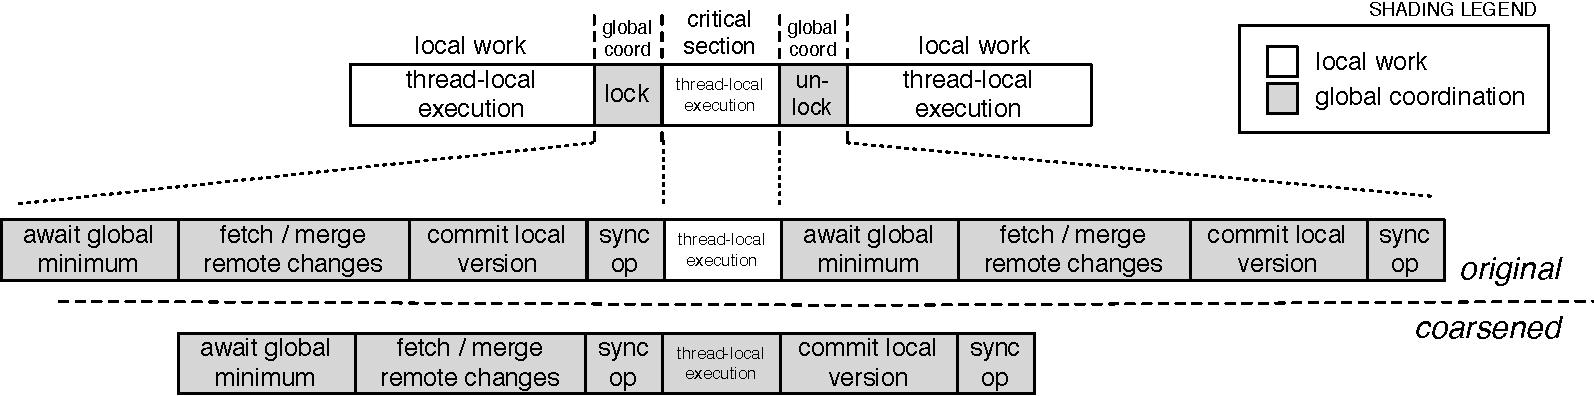
\includegraphics[width=6.8in]{figures/coarsening}
\caption{Program execution under \lib{} is divided into phases of local work and global coordination. In this example, a critical section is surrounded by two phases of global coordination, for the lock and unlock operations respectively. The lower part of the figure shows the result of coarsening on this example.}
\label{f:coarsening}
\end{figure*}

Fig. \ref{f:coarsening} illustrates the operation of \lib{} for a critical section. In the local work phase, all changes are made to the local copy. When a synchronization operation is reached, the thread enters the global coordination phase. It sleeps until it has the global minimum instruction count (GMIC) and can acquire the token, then retrieves any remote updates, and commits its own changes before acquiring the lock. It then releases the token and begins its critical section. The critical section constitutes another local work chunk, which is followed by another global coordination phase. 

From this example, it is clear that though the work performed in the global coordination phase may be highly optimized, each deterministic synchronization operation will incur substantial overhead vs. its nondeterministic equivalent. This problem becomes particularly severe when the time between synchronization operations is brief, such that the local work is dwarfed by the global coordination surrounding it. 

To address this problem, we propose to adaptively reduce the number of global coordination phases, through a technique we call coarsening. In essence, coarsening combines several global coordination phases into a single phase, which includes the intervening local work chunks. The lower part of Fig. \ref{f:coarsening} illustrates the effect of coarsening on a single critical section. Here, the coordination work required is substantially reduced, at the cost of moving what used to be (parallel) local work into the (serialized) global coordination phase. 
As discussed in more detail below, coarsening is not limited to pairs---any number of local work chunks and their surrounding coordination may be coarsened into a single, longer global coordination phase. 

%Recall that a {\it chunk} is a unit of local work that appears between global synchronization phases. 
%When the chunk length is short, the cost of a \lib{} memory fence can become the dominating factor in program execution time. Each memory fence must read the performance counter, wait until its DLC is the global minimum, acquire/release the token and invoke \conversion{} to commit/update/merge memory. For this reason, short chunks can create a significant amount of sequential overhead.

%\TODO{this reads as if we're doing coarsening for everything, but in fact the only coarsening candidates are lock and unlock}

%We can reduce the number of memory fences by coarsening the chunks, creating longer chunk lengths that can effectively mask the overhead of a fence. 
While this technique sounds straightforward, several challenges arise. First, in order to maintain TSO consistency, other threads are blocked at their next synchronization operation until the coarsened chunk has completed. This means that an overly ambitious coarsening policy, producing excessively long coarsened chunks, can significantly harm the overall system by causing excessive waiting of other threads. Second, the choice of when to begin a coarsened chunk must be an informed one. If \lib{} chooses to coarsen and the next chunk is very long (which cannot be known ahead of time) the result would be a net loss in performance. Finally, these decisions need to be done deterministically.

Our approach is to use an adaptive coarsening policy that estimates, for each synchronization variable, the next chunk length using an exponentially weighted moving average of earlier chunk lengths. One such estimate is maintained per lock, for use with coarsening $lock$ operations, and a thread-local estimate is maintained for use with coarsening $unlock$ operations.  
%On completion of a chunk we add the length to a thread-local exponentially weighted moving average (EWMA). Before we execute a memory fence and begin the next chunk we consult the EWMA for a guess of what the next chunk length will be. 
Coarsening proceeds until either (a) the estimated total coarsened chunk length exceeds a maximum threshold, or (b) a conditional variable or barrier operation is encountered. 
%If $current\_length+chunk\_length\_estimate < max\_coarsening\_length$ then we will elide the memory fence and continue. 
%For more accurate statistics we use the synchronization variable as additional context by storing per-variable EWMA's. 

We deterministically adapt the maximum chunk length at runtime, using a multiplicative increase, multiplicative decrease policy. 
Each time a thread $T1$ enters the global coordination phase, $T1$ compares its thread id to the id of the thread $T2$ that previously entered the global coordination phase.
If $T1==T2$, the maximum chunk length is doubled. Conversely, if $T1\neq{}T2$, the maximum chunk length is halved. 
This allows each thread to individually adapt to current conditions.
Because all decisions are based on chunk lengths and the token order, both of which are deterministic, coarsening maintains determinism.

\subsection{Adaptive Counter Overflows}

A thread's logical clock can be updated primarily in one of two ways: (1) when a thread finishes a chunk and the performance counter is read and (2) when a performance counter overflows, triggering an interrupt. Regarding the latter, the choice of overflow frequency is a trade-off between sequential overhead and logical clock accuracy. With a low frequency of overflows, a thread that is not the GMIC may wait longer to receive the notification that they are the new global minimum. However, if the frequency is too high, the cost of exception handling can become unwieldy (see \cite{olszewski_kendo:_2009} for further discussion). 

Our solution to this problem is based on the observation that overflow frequency does not impact determinism at all. A lower or higher frequency may impact when a thread is notified in real time, but it has no bearing in logical time. Therefore,  we design our logical clock module to adapt our overflow frequency using three simple rules. First, at the beginning of each chunk, the overflow is set to a conservative base value of 5,000 retired instructions. Second, if we are the GMIC, then at the beginning of each chunk and at each overflow we check to see if the next lowest logical clock is currently waiting to become the GMIC. If so, we set the performance counter to overflow just when our clock exceeds theirs. Third, if there is not a thread that we must notify then we double the number of instructions that will occur before the next overflow. 

%\subsection{Other Optimizations}

\subsection{Thread Reuse for Fork-Join Programs}

In order to support fork-join concurrency it is imperative for \lib{} to provide fast thread creation and tear-down. However, the use of processes with \conversion{} memory makes this a challenging goal. When a new thread is spawned the call is intercepted by \lib{} and instead a new process is forked (\S\ref{s:isolation}). Because \conversion{} memory is mapped as a private segment, each populated page-table entry in the \conversion{} segment must be copied into the child's page-table. Depending on the application, this can be a large number of entries to copy and adds a significant amount of latency to thread creation. To help mitigate this issue, \lib{} keeps a pool of threads that have recently finished executing. When spawning a new thread, if a thread is waiting in the pool that thread is reused, eliminating an expensive fork operation. The newly spawned thread will still have to update its view of memory to reflect what has been committed since it began waiting in the pool. However, this is typically a much cheaper operation than forking a new process.

\subsection{User Space Reading of Performance Counters}

Our deterministic logical clock module resides primarily in the kernel. One advantage of this approach is that performance counter overflows that identify a new GMIC can notify waiting threads directly from kernel space using shared memory, avoiding costly signals to user space for each overflow. There is added cost to this design however, as \lib{} would require system calls at the end of each chunk to read the counters and determine (and potentially notify) a newly-appointed GMIC thread. To avoid the system call latency for short chunks, we allow user space reading of the performance counters when executing a coarsened chunk.

\lstset{numbers=left,language=C, basicstyle={\footnotesize\ttfamily},tabsize=1,frame=shadowbox,linewidth=7cm,numbers=left}

\newsavebox{\mutexLock}
\begin{lrbox}{\mutexLock}% Store first listing
\begin{lstlisting}
void mutexLock(lock_t* l){
	clockPause();
	while(true){
		waitToken();
		if (lockAcq(l)){;
			convCommitAndUpdateMem();
			break;
		}
		else{
			clockDepart();
			insert(l->waitQueue, _tid);
			releaseToken();
			waitForRelease(l);
		}
	}
	releaseToken();
	clockResume();
}
\end{lstlisting}
\end{lrbox}


\newsavebox{\waitToken}
\begin{lrbox}{\waitToken}% Store first listing
\begin{lstlisting}
void waitToken(){
	while(!isGMIC() || token!=NULL){}
	token=_tid;
}

void releaseToken(){
	token=NULL;
}
\end{lstlisting}
\end{lrbox}

\begin{figure}
\hspace*{.5cm}
\usebox{\mutexLock}
\caption{mutexLock() implementation.}
\label{f:mutexLock}
\end{figure}


\begin{figure}
\hspace*{.5cm}
\usebox{\waitToken}
\caption{A simplified implementation of token acquisition and release.}
\label{f:waitToken}
\end{figure}


\subsection{Fast Forward}
\label{s:fast-forward}

A thread may wait on a conditional variable or lock for an indefinite amount of time, causing its logical clock to become further and further behind the rest of the threads in the system. When the thread is finally woken and acquires the token, it may be the GMIC thread for a long time to come. To combat this, \lib{} ``fast forwards'' a thread's logical clock to the value of the logical clock of the last thread to release the token if that thread had a larger clock.\footnote{Kendo \cite{olszewski_kendo:_2009} employed a similar mechanism to avoid excessive logical clock increments in their locking algorithm.} 

%%% Local Variables: 
%%% mode: latex
%%% TeX-master: "paper.tex"
%%% End:


{\footnotesize \bibliographystyle{acm}
\bibliography{../common/bibliography}}


\theendnotes

\end{document}








